% =====================================================================
%  TFG - Grado en Ingeniería Multimedia - EPS Universidad de Alicante
%  Compilar:  latexmk -pdf main.tex      (pdflatex + biber)
% =====================================================================
\documentclass[12pt,a4paper,twoside,openright]{book}

% =====================================================================
%  ESTILO  -  Libro de Estilo TFG/TFM, EPS Universidad de Alicante
% =====================================================================

% --- Idioma y codificación -------------------------------------------
\usepackage[T1]{fontenc}
\usepackage[utf8]{inputenc}
\usepackage[spanish,es-tabla,es-nodecimaldot]{babel} % "Tabla" en vez de "Cuadro"
\addto\captionsspanish{%
  \renewcommand{\contentsname}{Índice de contenidos}%
  \renewcommand{\listfigurename}{Índice de figuras}%
  \renewcommand{\listtablename}{Índice de tablas}%
  \renewcommand{\appendixname}{Anexo}%
}

% --- Tipografía (apdo. 1.2) ------------------------------------------
% Familia 2 (texto) y fórmulas: Palatino (matemáticas en Palatino itálica)
\usepackage[sc]{mathpazo}
\linespread{1.05}
% Familia 1 (títulos y bibliografía): Helvética
\usepackage[scaled=0.92]{helvet}
% Familia 3 (código, ancho fijo): Courier
\usepackage{courier}
\usepackage{microtype}

% --- Página, márgenes e interlineado (apdo. 1.3 y 1.4) ---------------
% Interior 3 cm, exterior 2,5 cm, superior/inferior 2,5 cm,
% cabecera y pie DENTRO del margen (includeheadfoot)
\usepackage[a4paper,
            inner=3cm, outer=2.5cm, top=2.5cm, bottom=2.5cm,
            includeheadfoot, headheight=15pt]{geometry}
\usepackage{setspace}
\onehalfspacing                          % interlineado 1,5
\usepackage{emptypage}                   % páginas en blanco sin cabecera

% --- Colores, gráficos ------------------------------------------------
\usepackage{xcolor}
\usepackage{graphicx}
\graphicspath{{imagenes/}}
\usepackage{tikz}
\usetikzlibrary{calc,babel}
\usepackage{booktabs}
\usepackage{array}
\usepackage{tabularx}
\newcolumntype{Y}{>{\raggedright\arraybackslash}X}
\usepackage{enumitem}
\usepackage{csquotes}

% --- Títulos de secciones en Familia 1 (Helvética) --------------------
\usepackage{titlesec}
\titleformat{\chapter}[display]
  {\sffamily\bfseries\huge}
  {\Large\chaptertitlename\ \thechapter}{8pt}{\Huge}
\titleformat{name=\chapter,numberless}[display]
  {\sffamily\bfseries\Huge}{}{0pt}{}
\titlespacing*{\chapter}{0pt}{0pt}{30pt}
\titleformat*{\section}{\sffamily\bfseries\Large}
\titleformat*{\subsection}{\sffamily\bfseries\large}
\titleformat*{\subsubsection}{\sffamily\bfseries\normalsize}
\setcounter{secnumdepth}{3}              % numeración arábiga 1.1.1
\setcounter{tocdepth}{2}

% Índices también con títulos en Familia 1
\usepackage{tocloft}
\renewcommand{\cftchapfont}{\sffamily\bfseries}
\renewcommand{\cftchappagefont}{\sffamily\bfseries}
\renewcommand{\cfttoctitlefont}{\sffamily\bfseries\Huge}
\renewcommand{\cftloftitlefont}{\sffamily\bfseries\Huge}
\renewcommand{\cftlottitlefont}{\sffamily\bfseries\Huge}

% --- Cabeceras diferenciadas páginas pares/impares (apdo. 1.4) --------
\usepackage{fancyhdr}
\pagestyle{fancy}
\fancyhf{}
\renewcommand{\chaptermark}[1]{\markboth{#1}{}}
\renewcommand{\sectionmark}[1]{\markright{\thesection\ #1}}
\fancyhead[LE]{\sffamily\small\nouppercase{\leftmark}}   % par: capítulo
\fancyhead[RO]{\sffamily\small\nouppercase{\rightmark}}  % impar: sección
\fancyfoot[LE,RO]{\sffamily\small\thepage}               % nº en lado exterior
\renewcommand{\headrulewidth}{0.4pt}
\fancypagestyle{plain}{\fancyhf{}%
  \fancyfoot[LE,RO]{\sffamily\small\thepage}%
  \renewcommand{\headrulewidth}{0pt}}

% --- Figuras y tablas (apdo. 4) ---------------------------------------
\usepackage[font=small,labelfont=bf,labelsep=colon]{caption}
% Nota obligatoria con la fuente bajo cada figura/tabla (apdo. 4.3)
\newcommand{\fuente}[1]{%
  \par\vspace{2pt}{\centering\footnotesize\textit{Fuente:} #1\par}}

% --- Código (Familia 3) ----------------------------------------------
\usepackage{listings}
\renewcommand{\lstlistingname}{Código}
\renewcommand{\lstlistlistingname}{Índice de códigos}
\lstset{
  basicstyle=\ttfamily\small\singlespacing,
  keywordstyle=\bfseries\color{blue!60!black},
  commentstyle=\itshape\color{gray},
  stringstyle=\color{red!50!black},
  numbers=left, numberstyle=\tiny\color{gray},
  frame=single, rulecolor=\color{gray!50},
  breaklines=true, showstringspaces=false,
  tabsize=2, captionpos=b,
  literate={á}{{\'a}}1 {é}{{\'e}}1 {í}{{\'i}}1 {ó}{{\'o}}1 {ú}{{\'u}}1
           {Á}{{\'A}}1 {É}{{\'E}}1 {Í}{{\'I}}1 {Ó}{{\'O}}1 {Ú}{{\'U}}1
           {ñ}{{\~n}}1 {Ñ}{{\~N}}1 {ü}{{\"u}}1 {¿}{{?`}}1 {¡}{{!`}}1
}

% --- Abreviaturas y siglas (apdo. 2.5) --------------------------------
\usepackage[printonlyused]{acronym}

% --- Bibliografía (apdo. 2.8): APA, en Familia 1 ----------------------
% Para sistema numérico (ISO 690): style=iso-numeric (paquete biblatex-iso690)
\usepackage[backend=biber, style=apa]{biblatex}
\addbibresource{bibliografia.bib}
\renewcommand*{\bibfont}{\sffamily\small}

% --- Enlaces (siempre lo último) --------------------------------------
\usepackage[colorlinks=true, linkcolor=black, urlcolor=blue!60!black, citecolor=blue!60!black]{hyperref}

% --- Páginas preliminares (apdo. 2.3 y 2.4) ---------------------------
% Una sola hoja, alineación derecha, distribuida verticalmente
\newenvironment{paginaderecha}
  {\cleardoublepage\thispagestyle{empty}\vspace*{\fill}\begin{flushright}\itshape}
  {\end{flushright}\vspace*{\fill}\clearpage}

% Capítulo sin numerar que sí aparece en el índice
\newcommand{\capitulosinnumero}[1]{%
  \chapter*{#1}\addcontentsline{toc}{chapter}{#1}\markboth{#1}{#1}}

% añadido
\usepackage{float}
% =====================================================================
%  DATOS DEL TFG  ->  Edita solo este archivo para la portada
% =====================================================================
\newcommand{\tituloTFG}{Desarrollo de un videojuego\\narrativo en 2D con mecánicas\\adaptativas sobre la\\perspectiva de género}
\newcommand{\tituloTFGpdf}{Desarrollo de un videojuego narrativo en 2D con mecánicas adaptativas sobre la perspectiva de género}
\newcommand{\titulacion}{Grado en Ingeniería Multimedia}
\newcommand{\tipoTrabajo}{Trabajo Fin de Grado}
\newcommand{\autorTFG}{Leigh Garrett}
\newcommand{\tutoresTFG}{Carlos J. Villagrá Arnedo\\Patricia Maria Compañ Rosique}   % varios: Nombre 1\\Nombre 2
\newcommand{\etiquetaTutor}{Tutor/es:}
\newcommand{\fechaTFG}{Junio 2027}              % "Mes Año"

% Color de la titulación (tabla del apdo. 1.7 del libro de estilo)
% Grado en Multimedia: RGB (239, 206, 53)
\definecolor{colorTitulacion}{RGB}{239,206,53}
% Texto sobre el color: negro en Multimedia (amarillo), blanco en colores oscuros
\definecolor{colorTextoPortada}{RGB}{0,0,0}
% Franja inferior oscura de la portada
\definecolor{colorFranja}{RGB}{35,31,32}


\hypersetup{pdftitle={\tituloTFGpdf}, pdfauthor={\autorTFG},
            pdfsubject={\tipoTrabajo. \titulacion}}

\begin{document}

% ---------------- Portada ----------------
% =====================================================================
%  PORTADA  (apdo. 1.7, figura 1 del libro de estilo)
%  Bloque superior 22,7 cm con el color de la titulación
%  Franja inferior 7,0 cm oscura
%  Logos en imagenes/ (vale .pdf, .png o .jpg):
%    logo-eps        -> logo EPS con el texto "Escuela Politécnica Superior"
%    logo-titulacion -> logo del grado
%    logo-ua         -> logo Universidad de Alicante (versión blanca)
%  Si un logo no existe se muestra un hueco provisional.
% =====================================================================

% \siexistelogo{nombre}{si existe}{si no existe}
% Deja en \rutalogo el archivo encontrado
\newcommand{\siexistelogo}[3]{%
  \IfFileExists{imagenes/#1.pdf}{\def\rutalogo{#1.pdf}#2}{%
  \IfFileExists{imagenes/#1.png}{\def\rutalogo{#1.png}#2}{%
  \IfFileExists{imagenes/#1.jpg}{\def\rutalogo{#1.jpg}#2}{#3}}}}

\begin{titlepage}
\newgeometry{margin=0cm}
\singlespacing
\begin{tikzpicture}[remember picture, overlay]
  % Bloque superior: color de la titulación
  \fill[colorTitulacion] (current page.north west)
       rectangle ([yshift=7cm]current page.south east);
  % Franja inferior
  \fill[colorFranja] (current page.south west)
       rectangle ([yshift=7cm]current page.south east);

  % --- Logo EPS (arriba derecha)
  \siexistelogo{logo-eps}{%
    % La imagen ya incluye el texto "Escuela Politécnica Superior"
    \node[anchor=north west, inner sep=0pt]
      at ($(current page.north west)+(13.4cm,-1.3cm)$)
      {\includegraphics[width=5.4cm]{\rutalogo}};
  }{%
    % Provisional: hueco + texto en Helvética 14 pt
    \node[anchor=north east, inner sep=0pt, text=colorTextoPortada]
      at ($(current page.north west)+(15.9cm,-1.4cm)$)
      {\fbox{\parbox[c][1.6cm][c]{2.1cm}{\centering\tiny logo EPS}}};
    \draw[colorTextoPortada, line width=1.2pt]
      ($(current page.north west)+(16.15cm,-1.3cm)$) -- ++(0,-1.9cm);
    \node[anchor=north west, align=left, inner sep=0pt,
          font=\fontfamily{phv}\fontsize{14}{16.5}\selectfont, text=colorTextoPortada]
      at ($(current page.north west)+(16.4cm,-1.45cm)$)
      {Escuela\\Politécnica\\Superior};
  }

  % --- Título: Helvetica Condensed 55 pt
  \node[anchor=north west, align=left, inner sep=0pt, text width=17.5cm,
        font=\fontfamily{phv}\fontseries{c}\fontsize{55}{62}\selectfont,
        text=colorTextoPortada]
    at ($(current page.north west)+(2.1cm,-9.6cm)$) {\tituloTFG};

  % --- Logo titulación + nombre de la titulación en Helvética 20 pt
  \siexistelogo{logo-titulacion}{%
    \node[anchor=west, inner sep=0pt] at ($(current page.north west)+(2.3cm,-15.3cm)$)
      {\includegraphics[width=2cm]{\rutalogo}};
  }{%
    \node[anchor=west, inner sep=0pt] at ($(current page.north west)+(2.3cm,-15.3cm)$)
      {\tikz\draw[colorTextoPortada, dashed] (0,0) circle (0.95cm);};
  }
  \node[anchor=west, inner sep=0pt,
        font=\fontfamily{phv}\fontsize{20}{24}\selectfont, text=colorTextoPortada]
    at ($(current page.north west)+(4.8cm,-15.3cm)$) {\titulacion};

  % --- Franja inferior: tipo de trabajo (20 pt) y datos (12 pt)
  \node[anchor=north west, inner sep=0pt,
        font=\fontfamily{phv}\fontsize{20}{24}\selectfont, text=white]
    at ($(current page.south west)+(2.4cm,5.95cm)$) {\tipoTrabajo};
  \node[anchor=north west, align=left, inner sep=0pt,
        font=\fontfamily{phv}\fontsize{12}{14.5}\selectfont, text=white]
    at ($(current page.south west)+(2.4cm,4.55cm)$)
    {Autor:\\\autorTFG\\[9pt]\etiquetaTutor\\\tutoresTFG\\[9pt]\fechaTFG};

  % --- Logo Universidad de Alicante (versión blanca)
  \siexistelogo{logo-ua}{%
    \node[anchor=south east, inner sep=0pt]
      at ($(current page.south west)+(19.4cm,1.5cm)$)
      {\includegraphics[width=6.4cm]{\rutalogo}};
  }{%
    \node[anchor=south east, inner sep=0pt, text=white]
      at ($(current page.south west)+(19.4cm,1.5cm)$)
      {\parbox{6.2cm}{\raggedleft\fontfamily{ptm}\fontsize{14}{16}\selectfont
         Universitat d'Alacant\\Universidad de Alicante}};
  }
\end{tikzpicture}
\restoregeometry
\end{titlepage}


% ---------------- Parte preliminar (apdo. 2.1 - 2.5) ----------------
\frontmatter
\capitulosinnumero{Resumen}

Este documento se corresponde con el Trabajo de Fin de Grado del Grado en Ingeniería Multimedia de Leigh Garrett. El presente trabajo, titulado «Desarrollo de un videojuego narrativo en 2D con mecánicas adaptativas sobre la perspectiva de género» y realizado en el curso académico 2026-2027, ha sido supervisado y tutorizado por Carlos J. Villagrá Arnedo y Patricia María Compañ Rosique.
\\\\
En los últimos años, el videojuego se ha consolidado como un medio artístico y expresivo capaz de abordar temáticas profundamente humanas e introspectivas. El presente proyecto consiste en la conceptualización, diseño y desarrollo de un videojuego narrativo en 2D centrado en el agotamiento psicológico derivado de una crisis de identidad de género a causa del rechazo social e internalizado. A partir de la perspectiva de género, la obra emplea la metáfora de un escenario apocalíptico y la exploración de una serie de mundos abstractos para representar el esfuerzo constante por encajar en las expectativas normativas de la sociedad.
\\\\
La principal aportación técnica y de diseño del proyecto radica en la implementación de un sistema de jugabilidad dinámica (gameplay adaptativo) en segundo plano. Este módulo analiza continuamente el comportamiento y las acciones del jugador durante la partida (identificando tendencias agresivas, pasivas o evasivas) con el fin de modificar dinámicamente las mecánicas, las habilidades del protagonista e incluso la propia interfaz gráfica de usuario (UI), reflejando así el estado psicológico interno del personaje. Con el propósito de evitar la frustración y garantizar la agencia del usuario, dicho sistema solicita el consentimiento explícito del jugador antes de aplicar las transformaciones en la experiencia de juego. Asimismo, para tratar estas cuestiones con el rigor y la sensibilidad necesarios, el proyecto contempla el asesoramiento de especialistas en el área de la psicología.
\\\\
El objetivo final del juego es sobrevivir a este viaje introspectivo hasta alcanzar un desenlace abierto, cuya naturaleza e interpretación dependerán directamente del vínculo construido entre el jugador y el protagonista a través de su estilo de juego. Esta memoria abarca desde el estudio del estado del arte y la fundamentación teórica sobre narrativa digital y mecánicas adaptativas, hasta la elaboración del Documento de Diseño de Juego (GDD), la dirección artística, la arquitectura técnica en el motor Unity y el desarrollo de un prototipo funcional y jugable.
\\\\
Palabras clave: Videojuego 2D, Narrativa Interactiva, Mecánicas Adaptativas, Perspectiva de Género, Salud Mental, Identidad de Género, Unity.
\capitulosinnumero{Justificación y objetivos}
%mas personal.
El presente Trabajo Fin de Grado surge de la necesidad de explorar nuevas formas de expresión interactiva en el medio del videojuego que integren el discurso narrativo directamente en sus mecánicas jugables. Aunque la industria independiente ha avanzado en la representación de temáticas introspectivas y de salud mental, gran parte de las obras actuales continúan separando la historia de la jugabilidad o implementan sistemas dinámicos que alteran las reglas de forma unilateral, generando frustración y pérdida de agencia en el usuario.
\\\\
Desde una perspectiva social, académica y técnica propia del Grado en Ingeniería Multimedia, este proyecto busca visibilizar el agotamiento psicológico derivado de una crisis de identidad de género a causa del rechazo social e internalizado. Para ello, se plantea el diseño y desarrollo en el motor Unity de un videojuego narrativo en 2D con vista cenital oblicua (\textit{top-down} 3/4) que emplea un sistema de mecánicas adaptativas en segundo plano y una mecánica de consentimiento explícito.
\\\\
El objetivo general del proyecto consiste en desarrollar un videojuego narrativo en 2D con un sistema de mecánicas adaptativas que explore una crisis de identidad desde la perspectiva de género, desglosándose en la elaboración del Documento de Diseño de Juego (\ac{GDD}) y su dirección artística con asesoramiento psicológico, la programación del módulo evaluador del comportamiento en segundo plano, la creación de una arquitectura flexible basada en \textit{ScriptableObjects} para mutar habilidades e interfaz (\ac{UI}) en tiempo real, y la construcción de un prototipo funcional y jugable.
\chapter*{Agradecimientos}
\markboth{Agradecimientos}{Agradecimientos}

Agradecimientos a las personas, entidades y organismos colaboradores.

\begin{paginaderecha}
A mi familia,\\
por su apoyo incondicional.
\end{paginaderecha}
   % opcional (una hoja)
\begin{paginaderecha}
\enquote{La simplicidad es la máxima sofisticación.}\\[6pt]
\upshape--- Autor de la cita
\end{paginaderecha}
          % opcional (una hoja)

% Índices: cada uno empieza en página nueva, en este orden
\tableofcontents
\listoffigures
\listoftables
% \lstlistoflistings                 % descomenta si quieres índice de código
\chapter*{Índice de abreviaturas y siglas}
\markboth{Abreviaturas y siglas}{Abreviaturas y siglas}

% Úsalas en el texto con \ac{SIGLA}: la primera vez sale desarrollada,
% después solo la sigla. Con printonlyused solo aparecen las usadas.
\begin{acronym}[WebGL]
  \acro{API}{Interfaz de Programación de Aplicaciones}
  \acro{EPS}{Escuela Politécnica Superior}
  \acro{TFG}{Trabajo Fin de Grado}
  \acro{UX}{Experiencia de Usuario}
  \acro{GDD}{Game Design Document}
  \acro{UI}{Interfaz de Usuario}
  \acro{URP}{Universal Render Pipeline}
  \acro{2D}{dos dimensiones}
\end{acronym}


% ---------------- Cuerpo (apdo. 2.6 y 2.7) ----------------
\mainmatter
\chapter{Introducción}
\label{cap:introduccion}

En los últimos años, el videojuego ha evolucionado hasta consolidarse como un medio audiovisual y expresivo capaz de abordar vivencias íntimas y problemáticas sociales complejas, tales como la salud mental y la búsqueda de la identidad \parencite{bogost2011, navarro2023}. Dentro de este ámbito, la representación de una crisis de identidad desde la perspectiva de género permite trasladar al lenguaje interactivo el agotamiento psicológico derivado de las expectativas normativas y del rechazo social e internalizado.

Con frecuencia, los videojuegos abordan su carga narrativa mediante recursos pasivos que interrumpen la acción, manteniendo mecánicas estáticas que no reaccionan al estado emocional del protagonista \parencite{finestrat2018}. Asimismo, aquellos títulos que modifican sus reglas de forma oculta suelen provocar frustración en el jugador al arrebatarle el control de manera imprevista.

Como solución en este \ac{TFG}, realizado en la \ac{EPS}, se propone el diseño y desarrollo de un prototipo funcional en \ac{2D} donde un sistema en segundo plano analiza las tendencias conductuales del usuario (agresiva, pasiva o evasiva) y, mediante un mecanismo de consentimiento explícito, adapta en tiempo real las habilidades del avatar y la interfaz gráfica de usuario (\ac{UI}).

El presente documento se ha estructurado siguiendo las directrices del Libro de Estilo de la Escuela Politécnica Superior de la Universidad de Alicante \parencite{eps2015} y tomando como referencia la estructura habitual de las memorias del Grado en Ingeniería Multimedia \parencite{finestrat2018}:
\begin{itemize}
    \item \textbf{Capítulo 1. Introducción:} contextualiza la temática del proyecto, expone la problemática existente en la intersección entre narrativa interactiva y mecánicas de juego y presenta la solución propuesta.
    \item \textbf{Capítulo 2. Marco teórico o Estado del arte:} establece los fundamentos sobre narrativa digital, narrativa ambiental, ludología frente a narratología, salud mental desde la perspectiva de género y mecánicas adaptativas, analizando obras de referencia del sector.
    \item \textbf{Capítulo 3. Objetivos:} define el objetivo general del proyecto y desglosa los objetivos específicos técnicos y de diseño.
    \item \textbf{Capítulo 4. Metodología:} describe el procedimiento de trabajo seguido, desde la investigación documental y el asesoramiento psicológico hasta la elección y justificación tecnológica del motor Unity.
    \item \textbf{Capítulo 5. Diseño del Videojuego (GDD) y Dirección Artística:} recoge la especificación completa del diseño del juego, incluyendo la sinopsis, los mundos abstractos, las reglas del sistema adaptativo, el consentimiento del jugador y el documento de diseño artístico.
    \item \textbf{Capítulo 6. Arquitectura Técnica e Implementación:} documenta el diseño de la arquitectura en Unity, el módulo de evaluación en segundo plano y el desarrollo del prototipo funcional.
    \item \textbf{Capítulo 7. Conclusiones:} sintetiza el grado de cumplimiento de los objetivos planteados y expone las líneas de trabajo futuro tras el \ac{TFG}.
\end{itemize}
\chapter{Marco teórico o Estado del arte}
\label{cap:estado}

Introducción al marco teórico, justificación de la elección de los temas tratados y su relación con el proyecto. Se trata de un capítulo de investigación documental que sirve como base para la toma de decisiones de diseño y desarrollo del prototipo. Consta de cuatro secciones principales: fundamentos de la narrativa digital y videojuegos, salud mental y perspectiva de género en los videojuegos, sistemas de juego dinámicos y mecánicas adaptativas, y análisis de obras de referencia. Todas ellas se han seleccionado por su relevancia en relación con la problemática planteada y la solución propuesta, así como por su capacidad para proporcionar un marco conceptual sólido que guíe el diseño y desarrollo del prototipo.

\section{Fundamentos de la Narrativa Digital y Videojuegos}
Con la llegada de los medios interactivos, la estructura narrativa ha evolucionado hacia el concepto de la Narrativa Digital (\textit{Digital Storytelling}), definida como la práctica de combinar la narración con contenidos digitales (imágenes, sonido, vídeo e interactividad) para construir una obra con un fuerte componente emocional y una finalidad que a menudo va más allá del simple entretenimiento: concienciar, educar o generar empatía \parencite{navarro2023}. A diferencia de los medios tradicionales cuya lógica se fundamenta en la representación pasiva, los videojuegos permiten una interacción activa del jugador, integrando al usuario como un agente causal que ejecuta y habita el relato en tiempo real \parencite{gomez2026, hernandez2024}.

A la capacidad de los videojuegos para transmitir argumentos y persuadir mediante sus reglas y sistemas se la conoce como retórica procedimental, concepto que ha sido analizado por \textcite{bogost2011}.

Existen tres pilares esenciales en toda estructura narrativa digital \parencite{navarro2023}:
\begin{itemize}
  \item \textbf{Contenido narrativo y modelo de mundo:} diferencia la cronología de vivencias del protagonista de la trama mostrada al jugador. El mundo del juego representa el conflicto íntimo del personaje, empleando un entorno apocalíptico como alegoría de sus dilemas.
  \item \textbf{Tiempo y ritmo (\textit{pacing}):} relación entre el tiempo de la historia y el tiempo del relato, en este caso del videojuego.
  \item \textbf{Personajes:} el jugador debe poder identificarse con los problemas, dudas y el agotamiento vital del protagonista.
\end{itemize}

\subsection{Ludología, Narratología y Armonía Ludonarrativa}
La ludología y la narratología son dos enfoques complementarios en el estudio de los videojuegos \parencite{finestrat2018, hernandez2024}. Tradicionalmente, la ludología situó el centro de la experiencia en el sistema de reglas, la simulación de comportamientos y la capacidad de ejercer el control, mientras que la narratología se enfocó en la estructura dramática, los personajes y la estética de la historia \parencite{cuadrado2020, gomez2026}.

De la fricción o el equilibrio entre ambas dimensiones surgen dos fenómenos clave estudiados por \textcite{hernandez2024}: la \textit{disonancia ludonarrativa}, que se produce cuando la estructura narrativa y las mecánicas jugables entran en contradicción rompiendo el significado de ello \parencite{gomez2026, hernandez2024}, y la \textit{consonancia ludonarrativa} (o armonía ludonarrativa), que surge cuando existe una alta cohesión entre la historia que se desea contar y las mecánicas e interfaz (incluyendo elementos diegéticos), dando a la obra más profundidad y significado artístico \parencite{hernandez2024}. Asimismo, tal y como demuestran \textcite{hernandez2024}, incluso estas fricciones ludonarrativas pueden emplearse deliberadamente como un recurso poético y expresivo para despertar emociones concretas en el jugador.

En este proyecto, se busca alcanzar una consonancia ludonarrativa profunda mediante la implementación de mecánicas adaptativas e interfaces que reflejen el estado psicológico del protagonista y las decisiones del jugador, permitiendo que la narrativa y la jugabilidad se complementen y potencien mutuamente \parencite{hernandez2024}.

\subsection{Narrativa Ambiental y Metáfora Visual}
La narrativa ambiental y la metáfora visual son técnicas utilizadas en los videojuegos para contar historias y transmitir emociones a través del diseño del entorno y los elementos visuales \parencite{finestrat2018, boyero2025}. Estas técnicas permiten a los jugadores experimentar la trama de manera más inmersiva, apoyándose en la abstracción gráfica, el cierre visual y la ambigüedad perceptiva para que el usuario descubra e interprete progresivamente el mundo del juego como símbolo del conflicto mental del protagonista \parencite{boyero2025}.

Obras como \textit{Inside} \parencite{playdead2016} y \textit{Little Nightmares} \parencite{tarsier2017} emplean la narrativa ambiental y la metáfora visual para explorar temas de opresión, control y miedo, utilizando el diseño de niveles, la iluminación y los elementos visuales para crear una atmósfera que refleje los dilemas del protagonista y genere empatía en el jugador \parencite{boyero2025}.

Para lograr una narrativa ambiental efectiva, es fundamental considerar aspectos como la coherencia del mundo del juego, la simbología de los elementos visuales y la interacción del jugador con el entorno \parencite{finestrat2018, boyero2025}. En este caso, el mundo del juego se presenta como un entorno apocalíptico de zombies donde tras recibir un mordisco el protagonista empieza a tener alucinaciones y da lugar a entornos abstractos mutantes, que refleja los conflictos internos del protagonista relacionados con su identidad de género y salud mental, convirtiendo el espacio transitable en una representación simbólica de sus luchas internas.

\subsection{Empatía, Agencia e Identificación con el Personaje}
El presente proyecto busca fomentar la empatía, la agencia y la identificación del jugador con el protagonista del juego. Como señala \textcite{cuadrado2020}, resulta necesario reformular el concepto clásico de actuación o agencia (\textit{agency}): más allá de entenderla únicamente como libertad absoluta de control mecánico (agencia funcional), la agencia en los videojuegos narrativos se abre hacia una agencia afectiva o dramática (\textit{dramatic agency}) vinculada a la construcción de sentido y al compromiso emocional con el personaje y su historia \parencite{cuadrado2020, hernandez2024}.

En esta línea, \textcite{gomez2026} propone que la construcción de la identidad en el videojuego se forma a través de una «tríada ontológica» compuesta por el \textit{Jugador} (entidad real), el \textit{Personaje} (entidad diegética con su trasfondo) y el \textit{Avatar} (cuerpo digital mediador). A través de esta relación triádica surge una «identidad proyectiva» en la que el usuario vierte sus valores y gestiona su propio «yo» mediante la toma de decisiones, llegando a generar un «residuo identitario», que consiste en un sedimento cognitivo, empático y moral que perdura en la conciencia del jugador tras finalizar la sesión de juego \parencite{gomez2026}.

Asimismo, como advierte \textcite{gomez2026} al analizar la «paradoja de la desposesión», cuando un sistema toma completo control del avatar al usuario, se produce una crisis en la agencia y una sensación de alienación. Es precisamente para evitar esta ruptura no deseada por lo que el presente \ac{TFG} introduce el mecanismo de \textit{Consentimiento Explícito}, asegurando que la transformación del avatar y sus mecánicas sea consensuada con el jugador.

\section{Salud Mental y Perspectiva de Género en los Videojuegos}
El análisis de los videojuegos desde la perspectiva de género ha cobrado una notable fuerza académica y creativa en la última década. Más allá de analizar la representación cuantitativa de personajes en la industria, aplicar la perspectiva de género al diseño de un videojuego implica cuestionar cómo las estructuras sociales, los roles de género normativos y la cisnormatividad impactan en la subjetividad y en la salud mental de las personas. Al operar como un «laboratorio ontológico» protegido dentro del círculo mágico lúdico, el videojuego permite al jugador habitar y experimentar de forma encarnada la fragmentación psicológica, la disforia y la presión normativa que atraviesa el protagonista \parencite{gomez2026}.

\section{Sistemas de Juego Dinámicos y Mecánicas Adaptativas}
En la historia de los videojuegos, se han desarrollado diversos sistemas de juego dinámicos y mecánicas adaptativas que permiten responder a las acciones del jugador de manera personalizada. Estos sistemas pueden ajustar la dificultad, modificar la narrativa o alterar la experiencia de juego en función del comportamiento del usuario, validando su identidad operativa a través de la retroalimentación sistémica (\textit{feedback}) \parencite{gomez2026, hernandez2024}.

En \textit{Disco Elysium} \parencite{zaum2020}, por ejemplo, las decisiones del jugador afectan directamente a la narrativa y fragmentan el diálogo psicológico interno del personaje \parencite{gomez2026}, mientras que en \textit{Silent Hill: Shattered Memories} \parencite{climax2009}, el juego adapta su atmósfera y los encuentros según las reacciones del jugador. Por otro lado, \textit{Undertale} \parencite{fox2015} ofrece un sistema que registra las decisiones mecánicas del jugador para interpelar su responsabilidad ética y alterar la historia, los diálogos y la interfaz en consecuencia \parencite{gomez2026}, mientras que \textit{Tell Me Why} \parencite{dontnod2020} utiliza la narrativa y el diseño de personajes para explorar temas de identidad de género y salud mental. Asimismo, títulos como \textit{Inside} \parencite{playdead2016} y \textit{Little Nightmares} \parencite{tarsier2017} emplean la narrativa ambiental y la metáfora visual para transmitir emociones y contar historias profundas sin necesidad de diálogos \parencite{boyero2025}.

Por lo tanto, la implementación de sistemas de juego dinámicos y mecánicas adaptativas no solo mejora la experiencia del jugador, sino que también permite abordar temas complejos y sensibles de manera más efectiva, fomentando la empatía y la comprensión a través de la interacción lúdica \parencite{bogost2011, cuadrado2020, gomez2026}. En este contexto, se propone un sistema de juego que observe las acciones del jugador y modifique dinámicamente la experiencia —incluyendo la interfaz de usuario (\ac{UI}) como extensión del flujo de conciencia del avatar \parencite{gomez2026, hernandez2024} y las mecánicas— para reflejar el estado psicológico del protagonista.

\section{Análisis de Obras de Referencia}
Para fundamentar tanto el diseño artístico como el diseño técnico del proyecto, se han estudiado diversas obras de referencia que comparten puntos de contacto con este \ac{TFG}:
\begin{itemize}
  \item \textit{Undertale} \parencite{fox2015}: un ejemplo de cómo el sistema emplea la retórica procedimental para registrar las decisiones mecánicas del jugador (atacar, perdonar, huir), deconstruyendo las convenciones del género para alterar profundamente la narrativa, los diálogos e incluso la propia interfaz de usuario y las reglas del combate \parencite{gomez2026}.
  \item \textit{Silent Hill: Shattered Memories} \parencite{climax2009}: referente técnico fundamental en el uso de un sistema de perfilado psicológico en segundo plano. El juego observa silenciosamente qué objetos mira el jugador, cómo reacciona ante los peligros y cómo explora el escenario, modificando dinámicamente la estética del mundo, el aspecto de las criaturas y el desenlace de la historia.
  \item \textit{Tell Me Why} \parencite{dontnod2020}: un juego de aventuras narrativas que aborda temas de identidad de género y salud mental, utilizando la narrativa y el diseño de personajes para explorar la experiencia de una persona transgénero.
  \item \textit{Inside} \parencite{playdead2016}: un juego de plataformas y aventuras que utiliza la narrativa ambiental y la metáfora visual para contar una historia profunda y emocional sin necesidad de diálogos, explorando temas de opresión y control \parencite{boyero2025}.
  \item \textit{Little Nightmares} \parencite{tarsier2017}: un juego de aventuras y plataformas que utiliza la narrativa ambiental y la metáfora visual para crear una atmósfera inquietante y transmitir emociones a través del diseño de niveles y la interacción con el entorno \parencite{boyero2025}.
  \item \textit{Disco Elysium} \parencite{zaum2020}: un juego de rol que combina narrativa profunda con mecánicas adaptativas que representan la fragmentación psicológica del protagonista, permitiendo al jugador influir en la historia y en la configuración interna del personaje a través de sus decisiones \parencite{gomez2026}.
\end{itemize}
\chapter{Objetivos}

El objetivo principal de este Trabajo de Fin de Grado es lo siguiente: desarrollar un videojuego narrativo en 2D con un sistema de mecánicas adaptativas que explore una crisis de identidad desde la perspectiva de género. Surge de la intersección entre la ingeniería de software aplicada al entretenimiento interactivo y la capacidad expresiva del medio del videojuego para generar emptaía frente a realidades sociales complejas \parencite{bogost2011,navarro2023}. En consecuencia, el objetivo general del proyecto consiste en conceptualizar, diseñar y desarrollar un prototipo funcional de videojuego narrativo en \ac{2D} con perspectiva cenital oblicua (\textit{top-down} 3/4) en el motor Unity que, mediante la implementación de un sistema de mecánicas adaptativas en segundo plano y una mecánica de consentimiento explícito, permita al jugador experimentar la crisis de identidad de género del protagonista y sus consecuencias psicológicas derivadas del rechazo social e internalizado. A través de esta propuesta se busca alcanzar una armonía ludonarrativa profunda \parencite{hernandez2024}, logrando que las reglas del sistema, las habilidades del jugador y la interfaz gráfica de usuario (\ac{UI}) evolucionen de manera sincroniada con el estado anímico del protagonista sin interrumpir la jugabilidad \parencite{gomez2026}.

Para alcanzar de la mejor manera posible al objetivo final del tema planteado, se plantea los siguientes objetivos específicos:
\begin{itemize}
  \item \textbf{Realizar un estudio teórico previo y fundamentar la perspectiva psicológica del proyecto:} analizar la literatura académica sobre narrativa digital, narrativa ambiental, disonancia y consonancia ludonarrativa e identidad proyectiva \parencite{finestrat2018, hernandez2024, gomez2026}, complementando esta base documental con el asesoramiento de una especialista en psicología para garantizar un tratamiento riguroso, empático y libre de estereotipos sobre la disforia y el estrés de minorías.
  \item \textbf{Elaborar el Documento de Diseño de Juego (\ac{GDD}) completo:} definir formalmente la sinopsis argumental, la estructura de los tres mundos abstractos (\textit{Vecindad Urbana}, \textit{Laberinto Fracturado} y \textit{Azotea Libre}), las manifestaciones simbólicas del escrutinio social y el flujo de mecánicas adaptativas, estableciendo las reglas exactas que modulan la transición hacia el desenlace abierto de la obra.
  \item \textbf{Establecer la dirección artística y el diseño visual en \ac{2D} con sensación de profundidad (2.5D):} diseñar la identidad gráfica del prototipo inspirándose en referentes contemporáneos como \textit{Oxenfree} \parencite{nightschool2016}, \textit{Night in the Woods} \parencite{infinitefall2017} y \textit{Undertale} \parencite{fox2015}, especificando las paletas cromáticas evolutivas, el diseño minimalista del avatar y de los entornos, la ordenación espacial en el eje vertical (\textit{Y-Sorting}), la iluminación bidimensional (\ac{URP} 2D) y las variaciones visuales de la interfaz.
  \item \textbf{Programar un módulo evaluador del comportamiento en segundo plano:} implementar en lenguaje C\# un sistema observador desacoplado que recolecte métricas de juego de forma transparente durante la partida (tales como acciones de confrontación directa, tiempos de inmovilidad o maniobras de esquiva y rodeo), evaluando dinámicamente la tendencia conductual predominante del usuario (agresiva, pasiva o evasiva).
  \item \textbf{Desarrollar una arquitectura de software flexible y el mecanismo de Consentimiento Explícito:} construir una base de programación modular apoyada en objetos de datos (\textit{ScriptableObjects}) de Unity que permita inyectar y modificar en tiempo real tanto las habilidades del personaje como la disposición y opacidad de la \ac{UI} sin corromper el estado de la partida, integrando un panel de consulta que solicite el permiso del jugador antes de aplicar cada mutación mecánica.
  \item \textbf{Construir y validar un prototipo funcional y jugable (demo):} integrar los sistemas programados, los recursos artísticos y el diseño de niveles en un corte vertical (\textit{vertical slice}) ejecutable en PC, llevando a cabo pruebas de funcionamiento e iteración para verificar la estabilidad técnica de las transiciones adaptativas y sentar las bases para la futura expansión del videojuego tras el \ac{TFG}.
\end{itemize}

\chapter{Metodología}

Para el correcto desarrollo de este Trabajo Fin de Grado se ha establecido una metodología estructurada en cuatro fases incrementales, combinando la investigación teórica, la validación conceptual y el diseño artístico con el desarrollo iterativo de software. Este enfoque escalonado permite abordar las limitaciones de tiempo y recursos propias de un proyecto académico individual, asegurando que la arquitectura base sea sólida antes de proceder a la construcción del prototipo jugable.

\section{Fases de Desarrollo del Proyecto}
El flujo de trabajo proyectado abarca desde la conceptualización inicial hasta la validación de la demo funcional. En la Figura~\ref{fig:fases-metodologia} se muestra el esquema general de las etapas que articulan la metodología del proyecto.

\begin{figure}[H]
  \centering
  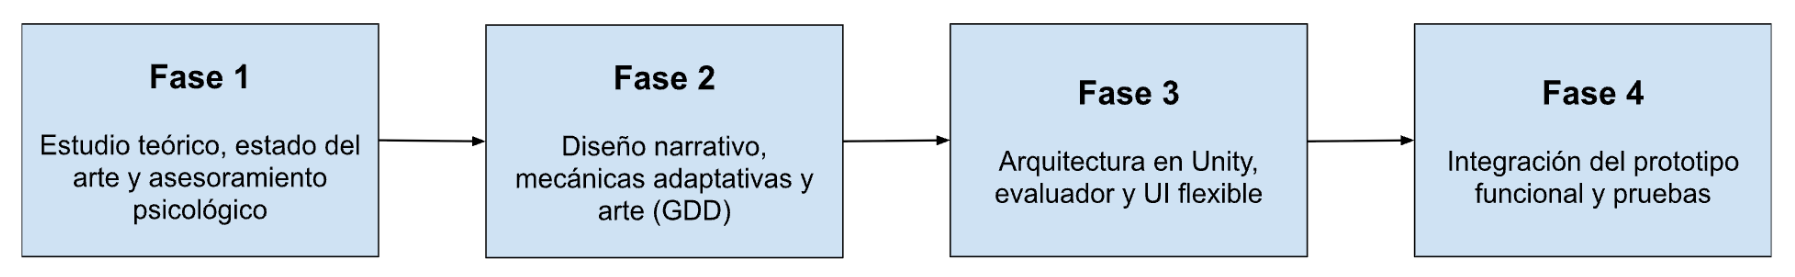
\includegraphics[width=0.8\textwidth]{fases.png}
  \caption{Diagrama de las fases incrementales de la metodología del proyecto}
  \label{fig:fases-metodologia}
  \fuente{elaboración propia}
\end{figure}

A continuación, se detalla el alcance y las tareas específicas que comprenden cada una de las cuatro etapas metodológicas:
\begin{enumerate}
  \item \textbf{Fase 1. Estudio teórico, documentación y asesoramiento psicológico:} el primer paso metodológico ha consistido en la revisión bibliográfica sobre narrativa digital \parencite{navarro2023}, narrativa ambiental \parencite{finestrat2018, boyero2025}, consonancia ludonarrativa \parencite{hernandez2024} y construcción de la identidad a través de la agencia \parencite{cuadrado2020, gomez2026}. Paralelamente, se han analizado obras de referencia que destacan bien por su tratamiento de la salud mental y la identidad como \textit{Celeste} \parencite{maddy2018}, \textit{Gris} \parencite{nomada2018}, \textit{Night in the Woods} \parencite{infinitefall2017} o \textit{Tell Me Why} \parencite{dontnod2020}, o bien por la utilización de sistemas de perfilado psicológico y adaptación al jugador como \textit{Silent Hill: Shattered Memories} \parencite{climax2009}, \textit{Undertale} \parencite{fox2015} o \textit{Disco Elysium} \parencite{zaum2020}. Asimismo, dado el compromiso del proyecto con la representación respetuosa de la perspectiva de género y la salud mental, esta fase incorpora sesiones de consulta y asesoramiento con una especialista en psicología con el fin de validar que la representación de la crisis identitaria y las estrategias de afrontamiento carezcan de estigmas o estereotipos dañinos. Para todas las referencias se ha adoptado la normativa estándar de citación APA conforme al Libro de Estilo de la \ac{EPS} \parencite{eps2015}.
  \item \textbf{Fase 2. Diseño narrativo, artístico y de mecánicas (\ac{GDD}):} a partir de las conclusiones extraídas en la investigación previa, se elabora el Documento de Diseño de Juego. En esta etapa se estructura el arco narrativo introspectivo dividido en tres mundos abstractos y las condiciones que modulan su desenlace abierto. En el plano mecánico, se definen los eventos concretos que alimentan el evaluador en segundo plano, las reglas de los mecanismos y la matriz de transformación de habilidades e interfaz. En el apartado visual, se establece la dirección artística en \ac{2D} con profundidad 2.5D bajo perspectiva cenital oblicua (\textit{top-down} 3/4), definiendo las paletas cromáticas evolutivas, el diseño de \textit{sprites} del avatar y de las manifestaciones abstractas, la iluminación ambiental y la maquetación de la interfaz adaptativa.
  \item \textbf{Fase 3. Desarrollo técnico de la arquitectura base en Unity:} antes de construir los niveles definitivos, el trabajo técnico se centra en programar los cimientos modulares del sistema en C\#. En primer lugar, se diseña una arquitectura desacoplada basada en eventos y contenedores de datos (\textit{ScriptableObjects}) capaz de modificar parámetros del jugador y del lienzo (\textit{Canvas}) en tiempo real sin comprometer la estabilidad de la ejecución. En segundo lugar, se implementa el módulo observador en segundo plano encargado de contabilizar las métricas de interacción del usuario y calcular los pesos conductuales que disparan las propuestas de adaptación.
  \item \textbf{Fase 4. Construcción iterativa del prototipo funcional y pruebas:} la última etapa aborda la construcción de un prototipo funcional jugable (demo o \textit{vertical slice}) que permita experimentar en la práctica la transición entre los estados del juego. Se integran las escenas en Unity, ordenación en el eje vertical (\textit{Y-Sorting}) e iluminación \ac{URP} \ac{2D}, procediendo finalmente a la realización de pruebas funcionales para verificar que la recolección de eventos, el panel de consentimiento y el cambio de habilidades funcionen de manera fluida.
\end{enumerate}

\section{Herramientas y Justificación Tecnológica}
Para llevar a cabo las distintas fases del proyecto se ha seleccionado el siguiente conjunto de herramientas de software:

\subsection{Motor Gráfico: Justificación de Unity}
El motor principal elegido para el desarrollo del videojuego es Unity \parencite{unity2023}. Su elección frente a otras alternativas del mercado responde a criterios técnicos alineados con los requisitos de este TFG:
\begin{itemize}
    \item Especializado en 2D: Unity cuenta con un conjunto de herramientas 2D maduras (\textit{Sprite Editor}, \textit{Tilemap}, \textit{2D Lighting}, animación por \textit{sprites}\ldots) \parencite{unity2023}, ideal para materializar la dirección artística de los mundos abstractos y las transiciones atmosféricas.
    \item Arquitectura basada en componentes y C\#: permite diseñar sistemas altamente modulares y orientados a eventos, y gracias a \textit{ScriptableObjects} facilita la creación de perfiles de habilidades e interfaces intercambiables en tiempo real sin acoplar clases ni afectar la estabilidad de la partida.
\end{itemize}

\subsection{Otras Herramientas empleadas}
\begin{itemize}
    \item Como IDE se utiliza Visual Studio para la codificación, depuración y refactorización de scripts en C\#.
    \item Para el control de versiones se utiliza Git y GitHub, que permite seguir el código fuente de manera segura.
    \item Para documentar se emplea LaTeX en Visual Studio Code, siguiendo la plantilla oficial de la Escuela Politécnica Superior \parencite{eps2015}.
\end{itemize}
\chapter{Diseño del Videojuego (GDD) y Dirección Artística}

Este capítulo recoge la especificación completa del diseño del juego, incluyendo la sinopsis, los mundos abstractos, las reglas del sistema adaptativo, el consentimiento del jugador y el documento de diseño artístico, que abarca el estilo visual, la paleta de colores, el diseño de personajes y entornos, la iluminación y la interfaz de usuario (UI) adaptativa. La justificación de las decisiones de diseño se fundamenta en la investigación documental y en el asesoramiento psicológico recibido durante la fase de desarrollo del proyecto, así como en la experiencia adquirida a lo largo del Grado en Ingeniería Multimedia. Además, se incluyen referencias a obras de videojuegos independientes y experimentales que han servido como inspiración para la creación de este prototipo funcional. Y como parte de la documentación del GDD, se presentan diagramas de flujo y tablas que ilustran la evolución de los perfiles conductuales del jugador y su impacto en la jugabilidad, así como la relación entre los elementos narrativos y las mecánicas adaptativas implementadas en el juego. En las referencias bibliográficas se incluyen fuentes académicas y artículos especializados que respaldan las decisiones de diseño y la implementación de mecánicas adaptativas en videojuegos, así como estudios sobre narrativa interactiva, salud mental y representación de género en medios digitales ya que estos aspectos son fundamentales para la comprensión del contexto y la relevancia del proyecto porque permiten situar el prototipo dentro de un marco teórico sólido y ofrecer una experiencia de juego que sea significativa y respetuosa con la temática abordada.

\section{Concepto General y Sinopsis Argumental}
Título del Proyecto: Sin definir
Género: aventura narrativa 2D / Exploración introspectiva
Plataforma Objetivo: PC / Mac (Entorno Unity)
Público Objetivo: jugadores interesados en experiencias narrativas independientes, representación LGTBIQ+, salud mental y diseño de juego experimental.

\subsection{Sinopsis}
El juego sitúa al personaje protagonista en el centro de un colapso apocalíptico. Lo que a primera vista aparenta ser la destrucción física de un mundo urbano decadente revela ser la representación externa del agotamiento mental causado por la disforia, la imposición de roles de género y el rechazo social acumulado. Para sobrevivir, el protagonista debe atravesar una serie de planos abstractos que personifican las etapas de su conflicto identitario, enfrentándose a manifestaciones físicas del escrutinio social y aprendiendo a reconocer su propio espacio e identidad.

\section{Diseño Narrativo y Estructura de Mundos Abstractos}
El desarrollo narrativo del juego se formula a través de tres mundos o dimensiones abstractas principales, cada una vinculada a un estado emocional y a un conjunto de estresores concretos:
\begin{itemize}
  \item Mundo 1: Vecindad Urbana: estructuras monolíticas, sombras fijas y entornos vacíos de vida. Simboliza la presión del entorno social y la necesidad forzada de adaptarse a expectativas externas. Las mecánicas iniciales son rígidas y restrictivas. Aquí el protagonista se enfrentará a dos manifestaciones abstractas: un ángel ciego y herido, y una entidad de la oscuridad sin cuerpo físico.
  \item Mundo 2: Laberinto Fracturado: escenarios fragmentados, flotantes, caracterizados por geometrías inestables y ecos sonoros, creando un especie de laberinto complicado. Representa la fase más crítica del agotamiento psicológico e internalizado. Aquí es donde el sistema adaptativo empieza a sugerir mutaciones profundas en el control del personaje y se enfrenta a dos manifestaciones abstractas: un amigo olvidado el cual busca que le encuentren, y un reflejo mutado del propio protagonista.
  \item Mundo 3: Azotea Libre: un plano de líneas depuradas, iluminación suave y espacio amplio. Esta etapa final es el desenlace que se adapta para ofrecer una resolución abierta cuyo tono e interpretación dependerá del perfil conductual consolidado a lo largo del juego. Aquí únicamente se dialogará directamente con el protagonista.
\end{itemize}

\section{Sistema de Mecánicas Adaptivas y Perfiles de Jugador}
El núcleo interactivo reside en la clasificación implícita de las acciones del jugador en tres perfiles conductuales:
\begin{itemize}
  \item Agresivo: realiza a menudo acciones de confrontación directa contra los obstáculos/enemigos, junto con un avance rápido seguido y uso frecuente de habilidades de impacto.
  \item Pasivo: se encuentra en largos periodos de inmovilidad ante la presencia de enemigos, avance lento, interacción cuidadosa con el entorno y casi nunca usa habilidades de impacto.
  \item Evasivo: uso constante de saltos, esquivas y rodeos para evitar contacto con posibles amenazas, teniendo una mínima interacción directa con el entorno.
\end{itemize}
A continuación, se muestra un esquema de flujo del sistema de mecánicas adaptativas:
\begin{figure}[H]
  \centering
  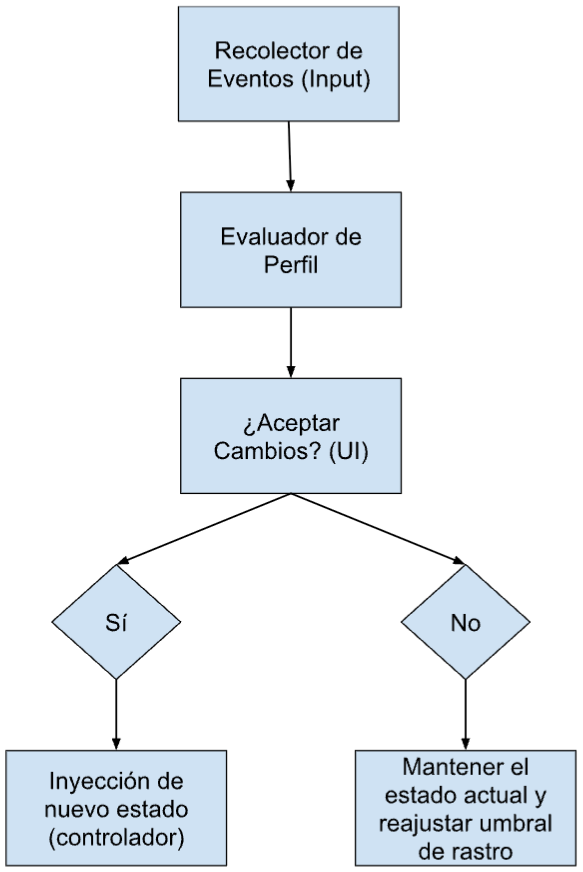
\includegraphics[width=0.8\textwidth]{Esquema.png}
  \caption{Esquema de flujo del sistema de mecánicas adaptativas}
  \label{fig:esquema-mecanicas}
  \fuente{elaboración propia}
\end{figure}
%lista de habilidades y transformaciones.
%NO ESTOY MUY SEGURO CON EL TEMA DE PERFILES, PUEDE ESTAR SUJETOS A CAMBIOS PEQUEÑOS O GRANDES.

\section{Consentimiento del Jugador y Accesibilidad Emocional}
A diferencia de otros títulos con sistemas de adaptabilidad oculta que modifican las reglas unilateralmente, este juego introduce la mecánica del Consentimiento Explícito. De tal manera que, cuando el analizador detecta un hábito consolidado a partir de las acciones optadas por el jugador, el juego presenta una notificación en pantalla donde el jugador puede seleccionar si aceptar la mutación de sus habilidades (por ejemplo, transformar esquivar en una carga frontal) o rechazar el cambio, conservando la configuración de control previa. Esta decisión garantiza que la agencia del usuario no sea vulnerada y evita la frustración mecánica, reforzando la idea de que la persona al mando tiene el control sobre el proceso de afrontamiento de su personaje.

\section{Documento de Diseño Artístico}
\subsection{Estilo Visual y Paleta de Colores}
La dirección artística opta por un estilo 2D con una marcada sensación de profundidad tridimensional (2.5D), articulado desde una perspectiva en tercera persona cenital oblicua (\textit{top-down} 3/4). Este enfoque visual toma como referentes principales la disposición espacial de \textit{Undertale} \parencite{fox2015}, junto con el acabado pictórico, atmosférico y estilizado de obras como \textit{Oxenfree} \parencite{nightschool2016} y \textit{Night in the Woods} \parencite{infinitefall2017}. De este modo, se evita el \textit{pixel art} convencional para construir entornos transitables en todas las direcciones del plano ($X$ e $Y$) que envuelven físicamente al protagonista.
\\\\
Esta identidad visual se fundamenta en tres pilares expresivos que refuerzan la metáfora del agotamiento psicológico y la crisis de identidad de género:
\begin{itemize}
  \item La cámara en ángulo picado oblicuo permite al jugador desplazarse libremente hacia el fondo, el frente y los laterales del escenario. A diferencia de una vista lateral plana, esta perspectiva subraya la vulnerabilidad del personaje al situarlo rodeado por la arquitectura opresiva y las manifestaciones del escrutinio social.
  \item Las figuras del plano jugable presentan siluetas vectoriales definidas y expresivas, mientras que los pavimentos en perspectiva, las estructuras colapsadas y los abismos emplean texturas orgánicas, pinceladas desgastadas y densos bancos de niebla que acentúan la perspectiva aérea y el aislamiento.
  \item La paleta cromática evoluciona según la carga emocional de la escena y la transición a través de los tres mundos abstractos (Tabla 1):
\end{itemize}
\begin{table}[H]
  \centering
  \caption{Paleta cromática de los entornos abstractos del juego y la evolución del UI.}
  \label{tab:paleta}
  \small
  \renewcommand{\arraystretch}{1.2}
  \begin{tabularx}{\textwidth}{YYYY}
    \toprule
    Entorno/Estado & Tono Dominante & Tono Secundario & Tono de Acento \\
    \midrule
    Mundo 1 &  & & \\
    Mundo 2 &  &  & \\
    Mundo 3 &  &  & \\
    \bottomrule
  \end{tabularx}
  \fuente{elaboración propia.}
\end{table}

\subsection{Diseño de Personajes y Entornos}
En primer lugar, en cuanto al personaje principal presenta un diseño minimalista de líneas fluidas y silueta andróginal, optimizado mediante sprites para asegurar su legibilidad en el plano bidimensional (X e Y) bajo la perspectiva cenital oblicua (top-down ¾). Siguiendo los principios de identificación empática \parencite{navarro2023}, se prescinde de rasgos faciales detallados, concentrando la expresividad en su postura corporal, el movimiento de su vestimenta y su sombra proyectada.
\\\\
Una vez que el jugador acepta un cambio, el aspecto del avatar muta en tiempo real según la Tabla 2
\begin{table}[H]
  \centering
  \caption{Evolución visual del protagonista según el perfil conductual consolidado.}
  \label{tab:EvolucionVisual}
  \small
  \renewcommand{\arraystretch}{1.2}
  \begin{tabularx}{\textwidth}{>{\raggedright\arraybackslash}p{2.5cm}YYY}
    \toprule
    Perfil Conductual & Silueta y Contorno & Animación y Postura Corporal & Tratamiento Cromático y Efectos \\
    \midrule
    Agresivo (Confrontación) & Cortes geométricos angulosos y trazo vectorial más grueso & Postura firme e inclinada hacia adelante en avances e impactos & Alto contraste respecto al pavimento y destellos de impacto\\
    Pasivo (Bloqueo) & Silueta compacta, encogida y de bordes redondeados & Avance lento, hombros retraídos y prenda replegada como refugio & Tonos desaturados que se mezclan con las sombras del entorno\\
    Evasivo (Huida) & Acabado liviano con bordes orgánicos difuminados & Movimiento ágil en saltos, esquivas y rodeos constantes & Estela traslúcida al cambiar rápidamente de dirección\\
    \bottomrule
  \end{tabularx}
  \fuente{elaboración propia.}
\end{table}

En segundo lugar, aplicando los principios de la narrativa ambiental \parencite{finestrat2018}, los escenarios y las entidades que los habitan proyectan el conflicto interno del protagonista sin recurrir a texto expositivo. Para materializar la profundidad tridimensional (2.5D) en Unity mediante \textit{Tilemap} y \textit{Sprite Editor} \parencite{unity2023}, cada escena combina un primer plano oclusivo (\textit{foreground}), un plano medio jugable con ordenación dinámica en el eje vertical (\textit{Y-Sorting}, permitiendo al avatar rodear obstáculos por delante y por detrás), y un fondo abisal con desplazamiento diferencial (\textit{parallax}).
\\\\
La distribución espacial de los tres mundos y el diseño de sus respectivas manifestaciones abstractas se organizan en la Tabla 3:
\begin{table}[H]
  \centering
  \caption{Diseño escenográfico y manifestaciones abstractas por mundos.}
  \label{tab:DiseñoEscenografico}
  \small
  \renewcommand{\arraystretch}{1.2}
  \begin{tabularx}{\textwidth}{>{\raggedright\arraybackslash}p{2.5cm}YYY}
    \toprule
    Entorno/Estado & Distribución espacial y recursos en Unity (2.5D) & Manifestaciones abstractas & Diseño visual de las manifestaciones \\
    \midrule
    Mundo 1 & Calles y plazas delimitadas por estructuras monolíticas y sombras fijas (Tilemap estático) & Ángel ciego y herido;Entidad de la oscuridad& El ángel emplea trazos vectoriales rígidos y agrietados; la entidad utiliza un espacio completamente oscuro sin contorno fijo desde donde únicamente se muestran sus manos\\
    Mundo 2 & Islas flotantes y geometrías inestables suspendidas sobre abismos (Parallax multicapa) & Amigo olvidado;Reflejo mutado del protagonista& El amigo presenta una silueta fragmentada y brumosa; el reflejo distorsiona el sprite del protagonista con proporciones quebradas\\
    Mundo 3 & Explanada amplia y despejada de líneas depuradas sin obstáculos restrictivos & Protagonista (diálogo interno) & Espacio abierto enfocado exclusivamente en la figura del propio avatar\\
    \bottomrule
  \end{tabularx}
  \fuente{elaboración propia.}
\end{table}

\subsection{Iluminación y Diseño de Interfaz (UI) Adaptativa}
En cuanto a la iluminación, para dotar al entorno cenital oblicuo (\textit{top-down} 3/4) de volumen sin sobrecargar el rendimiento ni complicar la jerarquía de Unity, se emplea el sistema \textit{2D Lighting} del paquete \textit{Universal Render Pipeline} (\ac{URP} 2D) \parencite{unity2023}, de tal manera que:
\\\\
Por un lado, en lugar de sistemas lumínicos dinámicos complejos, utilizan luces globales suaves (Global Light 2D) combinadas con luces puntuales fijas (Point Lights 2D) en puntos estratégicos de los escenarios para marcar zonas de interés o áreas de transición.
\\\\
Por otro lado, el avatar incorpora un único componente de luz puntual hijo de su jerarquía (Point Light 2D de corto alcance), lo que proyecta un halo circular continuo sobre el suelo a su alrededor sin requerir cálculos pesados de sombras en tiempo real, garantizando una ejecución fluida en el prototipo.
\\\\
En cuanto a la interfaz de usuario (UI) adaptativa se implementa mediante un único lienzo (Canvas) en espacio de pantalla con elemetnos dinámicos controlados por scripst ligeros. La ventana de notificación del Consentimiento Explícito se resuelve mediante un panel de diálogo flotante básico que pausa temporalmente la lógica de movimiento (Time.timeScale = 0), evitando la complejidad de gestionar interfaces completamente diegéticas en 3D.
\\\\
El cambio visual de los elementos de UI según el perfil detectado por el sistema en segundo plano se gestiona de forma eficiente mediante perfiles de datos (ScriptableObjects), adaptando sus parámetros visuales conforme a la Tabla 4:
\begin{table}[H]
  \centering
  \caption{Cambio visual de la interfaz de usuario (UI) según el perfil conductual evaluado.}
  \label{tab:CambioVisualUI}
  \small
  \renewcommand{\arraystretch}{1.2}
  \begin{tabularx}{\textwidth}{>{\raggedright\arraybackslash}p{2.5cm}YYY}
    \toprule
    Perfil conductual & Estilo Visual de la UI & Comportamiento en Pantalla & Nivel de opacidad y contraste \\
    \midrule
    Agresivo & Bordes angulosos y trazos destacados & Posición fija y estable en la esquina superior del lienzo & Opacidad alta y colores contrastados\\
    Pasivo & Líneas finas y formas compactas & Retraimiento visual hacia los márgenes de la pantalla & Opacidad reducida\\
    Evasivo & Trazos suaves y redondeados & Movimiento de flotación sútil adaptado al desplazamiento del avatar & Opacidad variable vinculada a la velocidad de movimiento\\
    \bottomrule
  \end{tabularx}
  \fuente{elaboración propia.}
\end{table}

% El código usa la familia de ancho fijo (código~\ref{lst:ejemplo}).
% \begin{lstlisting}[language=Java, caption={Ejemplo de función}, label={lst:ejemplo}]
% // Calcula la distancia entre dos puntos
% public double distancia(Punto a, Punto b) {
%     double dx = a.x - b.x;
%     double dy = a.y - b.y;
%     return Math.sqrt(dx * dx + dy * dy);
% }
% \end{lstlisting}

% \section{Ejemplo de fórmula}
% Las fórmulas sencillas en línea se escriben así: $x^2 + y^2 = r^2$, $a + b = c$.
% Las más complejas, numeradas:
% \begin{equation}
%   d(a,b) = \sqrt{(a_x - b_x)^2 + (a_y - b_y)^2}
%   \label{eq:distancia}
% \end{equation}

\chapter{Arquitectura Técnica e Implementación}

Resultados obtenidos, análisis y discusión de los mismos.

\chapter{Conclusiones}

Resumen de los objetivos conseguidos y de los resultados obtenidos.

\section{Trabajo futuro}
Posibles líneas de continuación.


% ---------------- Bibliografía (apdo. 2.8) ----------------
\cleardoublepage
\markboth{Bibliografía}{Bibliografía}
\printbibliography[heading=bibintoc, title={Bibliografía y referencias}]

% ---------------- Anexos (apdo. 2.9) ----------------
\appendix
\chapter{Manual de usuario}
\label{anx:manual}

Contenido del anexo.


\end{document}
